Методы вывода демографической истории популяций можно разделить на две группы, которые отличаются принципом метода настройки параметров модели.
Первая группа методов позволяет получить распределения для значений демографических параметров $\theta$, вторая группа предоставляет только точечную оценку $\theta$.
Данная работа сфокусирована на второй группе методов, однако, приведем обзор методов обеих групп.

Существует несколько методов~\cite{cornuet2014diyabc,gronau2011bayesian, hey2018phylogeny}, позволяющих получить распределения для значений параметров демографической истории популяций. 
Эти методы позволяют количественно оценить неопределенность в оценках демографических параметров и могут быть особенно полезны для вывода сложных демографических историй.
Они часто основаны на байесовском статистическом выводе, где задается априорное распределение вероятности $P(\theta)$ для неизвестных параметров $\theta$ и вероятность $P(\mathfrak{D} | \theta)$ наблюдаемых данных $\mathfrak{D}$.
Теорема Байеса позволяет вычислить апостериорное распределение параметров $P(\theta | \mathfrak{D})$ следующим образом:
$$P(\theta | \mathfrak{D}) = \frac{P(\mathfrak{D} | \theta) P(\theta)}{P(\mathfrak{D})},$$
где знаменатель $P(\mathfrak{D})$ может быть вычислен как нормирующая константа.
Полученное в результате апостериорное распределение $P(\theta | \mathfrak{D})$ представляет собой распределение для параметров модели демографической истории, которое учитывает данные, и является результатом работы первой группы методов.

Одним из методов, позволяющих найти апостериорное распределение является приближенное байесовское вычисление (Approximate Bayesian Computation, ABC).
В ABC методе, вместо вычисления точной вероятности данных при заданных параметрах модели, генерируются множества случайных значений параметров модели.
Затем выбираются только те параметры, которые производят данные, сходные с реальными наблюдениями.
С использованием выбранных параметров аппроксимируется вероятность $P(\theta | \mathfrak{D})$.
Другим не менее популярным методом является методы Монте-Карло с марковскими цепями (Markov chain Monte Carlo, MCMC), которые позволяют сэмплировать любую функцию распределения с использованием цепи Маркова.
Как и в случае с методом приближенного байесовского вычисления, методы MCMC позволяют построить выборку из распределения $P(\theta | \mathfrak{D})$. и затем аппроксимировать его по ней.
Например, в работе \cite{cornuet2014diyabc} представлен метод, основанный на приближенном байесовском вычислении для поиска апостериорных распределений на параметры демографической истории популяций, а в работах \cite{gronau2011bayesian, hey2018phylogeny} авторы используют методы Монте-Карло с марковскими цепями для решения той же задачи.






Одной из главных задач популяционной генетики является изучение процессов, приводящих к изменению генетического состава популяций со временем. Для этого используются различные модели, такие как модели Райта-Фишера, Морана или Кингсмана, которые описывают, как изменяются генетические частоты и генотипы в популяциях.

Задача поиска структуры популяций является важной в популяционной генетике.
Структура популяций означает, что они могут быть разделены на различные подгруппы, которые имеют уникальные генетические свойства и различную степень разнообразия.
Для решения задачи поиска структуры популяций используют различные методы, включая метод главных компонент (PCA), кластерный анализ, дискриминантный анализ, моделирование байесовской сети и многие другие. Эти методы позволяют выделить подгруппы популяций, определить структуру генетических кластеров и оценить степень разнообразия внутри и между популяциями.

Филогенетические деревья являются важным инструментом в популяционной генетике для изучения эволюционных связей между организмами и группами организмов. 
Они позволяют понять, какие виды и организмы находятся в наиболее близком родстве друг с другом, а также как эти организмы эволюционировали в процессе времени. 
Филогенетические деревья строятся на основе молекулярных данных, таких как последовательности ДНК или РНК, и могут быть использованы для решения различных биологических и медицинских задач. 
Например, они могут помочь в исследовании распространения инфекций или в поиске новых лекарственных препаратов.
Для построения филогенетических деревьев используются различные методы, такие как метод максимального правдоподобия, метод байесовской статистики, метод максимального парсимонии и другие.

Поиск демографической истории популяций также является важной задачей в популяционной генетике. 
Демографическая история отражает изменения численности популяции, миграции, подбор и другие факторы, которые влияют на генетическое разнообразие.
Изучение демографической истории позволяет понимать, как популяции адаптируются к изменяющимся условиям среды, как происходят эволюционные изменения и как распределяется генетическое разнообразие между популяциями.

Методы популяционной генетики находят широкое применение в различных областях науки и практики. 
Одной из главных областей применения является эволюционная биология, где популяционная генетика помогает понять процессы, связанные с силами эволюции.
Кроме того, методы популяционной генетики используются в исследованиях, связанных с сохранением и управлением биоразнообразием.
Они позволяют определить уровень генетического разнообразия и выявить потенциальные проблемы, связанные с его потерей в популяциях.
Также популяционная генетика применяется в медицине для изучения наследственных заболеваний, определения риска их возникновения и прогнозирования исхода болезней.
Другие области, где используются методы популяционной генетики, включают сельское хозяйство, экологию, генетику популяций животных и растений, антропологию и археологию.

В данной главе рассматриваются существующие методы для решения различных задач биоинформатики, включая задачу вывода демографической истории популяций.
В разделе~\ref{sec:part1:bioinf_methods} представлены основы методов машинного обучения, оптимизации и искусственного интеллекта, а также примеры их применения в биоинформатике.
Раздел~\ref{sec:part1:dem_inf} содержит введение в основные понятия биологии и генетики, включая определение демографической истории популяции и постановку задачи вывода этой истории по генетическим данным.
Также в разделе~\ref{sec:part1:dem_inf} представлен обзор существующих методов, используемых для решения этой задачи.
\\




В последние годы происходило активное развитие методов машинного обучения и искусственного интеллекта.
%В основе машинного обучения лежит идея обучения компьютерных систем на основе опыта, что позволяет им улучшать свою производительность с течением времени.
Методы искусственного интеллекта включают в себя обширный спектр алгоритмов, которые позволяют компьютерным системам смоделировать и эмулировать интеллектуальные функции,которые ранее были доступны только человеку.
Машинное обучение --- это область искусственного интеллекта, в которой компьютерные системы обучаются автоматически извлекать закономерности из данных, не явно заданных в программном коде.
Это достигается путем создания математических моделей, которые могут анализировать данные и делать прогнозы или принимать решения на основе обучения на предыдущих данных.

Модель в машинном обучении представляет собой алгоритм, который обрабатывает данные, чтобы получить желаемый результат.
Модель строится на основе набора данных, которые представляют собой тренировочный набор.
Модель обучается на этом наборе данных, чтобы извлекать общие закономерности, которые могут быть использованы для предсказания результатов на новых данных.

Классические задачи машинного обучения включают в себя классификацию, регрессию и кластеризацию.
Классификация --- это задача, в которой необходимо определить, к какому классу относится объект на основе его свойств.
Регрессия --- это задача, в которой необходимо определить значение переменной на основе других переменных. 
Кластеризация --- это задача группировки объектов на основе их сходства, без учета заранее заданных классов.

Одновременно с развитием методов машинного обучения и искусственного интеллекта происходило накопление большого объема генетических данных, что открывает новые возможности для ответа на фундаментальные биологические вопросы, которые ранее не могли быть решены~\cite{galperin2010complete}.
В связи с этим появилось множество методов обработки этих данных в области биоинформатики --- новой дисциплины, которая комбинирует математику, информатику и биологию~\cite{maloy2013brenner}.
Основными компонентами биоинформатики являются методы программного обеспечения, а также анализ и интерпретация биологических данных с помощью этих методов.
Биоинформатика позволяет дать ответы на многие вопросы биологии, включая геномику, генетику, транскриптомику, протеомику и фармакологию.

%\subsection{Методы машинного обучения в биоинформатике}

Интерпретация длинных последовательностей геномов может вызывать значительные вычислительные трудности.
Машинное обучение и искусственный интеллект используются в биоинформатике для обработки и анализа больших объемов биологических данных.
Машинное обучение может быть основано на различных алгоритмах, таких как метод опорных векторов, деревья решений, нейронные сети и многие другие.
С их помощью создаются модели, которые обучаются на основе набора данных и используются для предсказывания значений на новых данных.
Выбор алгоритма машинного обучения зависит от конкретной биологической задачи и доступного набора данных.

Машинное обучение может использоваться для различных задач биоинформатики, например, для классификации белков~\cite{diplaris2005protein}.
Белки являются ключевыми элементами во многих биологических процессах.
Классификация белков может помочь в определении их функций и свойств, а также в понимании механизмов болезней, связанных с дефектами белков.
Обученную модель классификации можно использовать для предсказывания функции нового ранее неизвестного белка.
В работе~\cite{diplaris2005protein} было представлено сравнение различных методов машинного обучения, включая деревья решений, метод k-ближайших соседей и метод опорных векторов, для решения задачи классификации белков.

Малые молекулы, которые могут связываться с белками, широко используются в фармакологии в качестве лекарственных препаратов.
Предсказание, насколько эффективно эти молекулы связываются с белками, позволяет сократить время и затраты на разработку новых лекарств, идентифицировать потенциальные цели для лечения болезней и повысить вероятность успеха клинических испытаний. 
Модель случайного леса может использоваться для обучения и предсказания степени связывания малых молекул с белками~\cite{ballester2010machine}.

Экспрессия генов --- это процесс, в результате которого информация, содержащаяся в гене, преобразуется в функциональный элемент --- РНК или белок. 
Выявление изменений в экспрессии генов может помочь в диагностике и лечении болезней.
Например, некоторые виды рака имеют специфические изменения в экспрессии генов, которые можно использовать для определения типа рака и выбора наиболее эффективного лечения.
Нейронные сети, такие как сеть радиально-базисных функций или многослойный перцептрон, а также другие методы машинного обучения могут использоваться для анализа данных генетической экспрессии и поиска изменений экспрессии у здоровых и больных людей~\cite{pirooznia2008comparative}.


Искусственный интеллект (Artificial Intelligence, AI) --- это область науки и технологий, которая занимается созданием алгоритмов и компьютерных систем, способных выполнять задачи, обычно требующие умственных способностей человека, таких как обучение, распознавание образов, анализ данных и принятие решений.
Все описанные ниже алгоритмы глобальной оптимизации могут лежать в основе методов искусственного интеллекта, так как они используют компьютерные алгоритмы, которые могут выполнять сложные задачи, требующие высокого уровня интеллекта.
Биоинформатика является областью, где применение алгоритмов глобальной оптимизации и искусственного интеллекта имеет широкие перспективы и может помочь в решении многих задач в биологии и медицине.



Классические алгоритмы оптимизации могут использоваться для настройки параметров различных моделей в области машинного обучения, а также биоинформатики.

Метод Бройдена, Флетчера, Голдфарба и Шанно (BFGS) широко используется наряду со своими модификациями. Например, в статье~\cite{ma2013protein} метод L-BFGS использовали для настройки весов нейронной сети, которая выполняла оценку вероятности локального выравнивания двух строк белков.
Информация, полученная от обученной нейронной сети, использовалась при построении выравнивания белков.
Метод выравнивания с использованием настроенной модели, предложенный в статье, позволяет выполнять более точный поиск белков с похожей структурой.
В~\cite{stewart2009application} авторы также использовали L-BFGS оптимизацию для настройки модели геометрической структуры больших молекул путем минимизации ее энергии.

Алгоритм Нелдера-Мида был использован в статье~\cite{nsoesie2013simulation}, где был предложен метод моделирования и прогнозирования динамики числа заболевших при эпидемии гриппа и других инфекционных заболеваний.
Модель симуляции эпидемии, предложенная авторами, учитывала такие параметры, как вероятность передачи, инкубационный и заразный периоды болезни, а также социальную сеть взаимодействий.
Для поиска оптимальных параметров модели был предложен алгоритм Нелдера-Мида, а в качестве целевой функции была рассмотрена среднеквадратичная ошибка между имеющейся кривой числа заболевших и предсказанной кривой за тот же промежуток времени.
Эффективность метода была продемонстрирована на симулированных данных для округа Монтгомери в Вирджинии, Майами и Сиэтла.
Найденная оптимальная модель успешно предсказала кривую эпидемии, время до пика, пиковое число и общее число инфицированных.

Как и метод BFGS, метод Пауэлла применяется для поиска трехмерной структуры молекул, например, в работе~\cite{loge2005three} его использовали для построения трехмерной структуры молекулы белка ароматазы, имеющей минимум энергии.
В работе~\cite{zhao2019design} оптимальные структуры химических соединений, полученные с помощью метода Пауэлла, использовали при разработке новых пестицидов, безопасных для пчел.




\emph{Метод имитации отжига} (Simulated Annealing)~\cite{metropolis1953equation,kirkpatrick1983optimization} ----- это стохастический метод оптимизации, использующий моделирование процесса отжига металла, при котором его структура меняется в зависимости от температуры.
В начале работы температура высока, что позволяет методу допускать переходы к более худшим решениям, тем самым уменьшая вероятность застревания в локальных оптимумах.
С каждой итерацией температура уменьшается, а с ней и вероятность принятия худшего решения, и алгоритм начинает сходиться к глобальному оптимуму.
Алгоритм продолжает работу до тех пор, пока температура не достигнет некоторой конечной точки останова или пока не будет достигнуто определенное число итераций.

Метод имитации отжига минимизирует функцию энергии $E(x) = -f(x)$ для определения качества решения $x$.
В процессе оптимизации, на каждой итерации, текущее решение $x$ заменяется на новое решение $x'$, которое получается из $x$ путем случайного изменения некоторых его параметров.
Далее, определяется изменение энергии $\Delta E=E(x')-E(x)$ между текущим и новым решением.
На основе значения $\Delta E$ и текущей температуры $T$, метод решает, принимать новое решение $x'$ или нет.
Если $\Delta E<0$, то новое решение принимается всегда, в противоположном случае, если $\Delta E>0$, то новое решение принимается с вероятностью $P=e^{-\Delta E/T}$, где $e$~--- число Эйлера.
С уменьшением температуры, вероятность принятия худшего решения уменьшается.
Ключевой составляющей метода является функция охлаждения, которая определяет, как быстро температура снижается в процессе оптимизации. Различные функции охлаждения могут использоваться в зависимости от типа задачи и требуемой точности.
Множество функций охлаждения используется для метода отжига, например, логарифмическое охлаждение~\cite{mahdi2017performance}:
$$T_{t} = \frac{c}{\log(1+t)},$$
где $T_{t}$ --- температура на итерации $t$, а $c$ --- положительная константа, независимая от $t$.
Еще одной часто используемой функцией охлаждения является линейное охлаждение, которое определяется следующим образом~\cite{mahdi2017performance}:
$$T_{t} = T_0 - \alpha t,$$
где $\alpha$ - коэффициент охлаждения.

Метод имитации отжига был предложен для решения биоинформатической задачи построения выравнивания нескольких последовательностей в работе~\cite{kim1994multiple}.
Выравнивание нескольких последовательностей --- важная задача биоинформатики, которая помогает в изучении молекулярной эволюции, а также в анализе отношений между структурой молекул и их последовательностями.
Обычно она решается методами динамического программирования, однако предложенный авторами метод имитации отжига позволяет снизить время вычислений, а также учитывать новые метрики оценки качества выравнивания.

\emph{Метод роя частиц} (англ. Particle Swarm Optimization)~\cite{kennedy1995particle,shi1998modified} является одним из методов глобальной оптимизации, который был предложен в 1995 году Кеннеди и Эберхартом. 
Метод моделирует поведение роя «частиц», которые движутся в пространстве поиска оптимального решения.
Каждая частица представляет собой потенциальное решение оптимизационной задачи, а её положение в пространстве определяется вектором $x_i = (x_{i,1}, x_{i,2}, \dots, x_{i,N})$, где $N$ - размерность пространства поиска, а $i$ - индекс частицы.
На каждой итерации $t$ алгоритма, каждая частица обновляет своё положение в пространстве поиска в зависимости от своего текущего положения и скорости, которая также представляется вектором $v_i = (v_{i,1}, v_{i,2}, \dots, v_{i,N})$.
Скорость и положение частиц изменяются следующим образом:
\begin{align*}
v_{i,j}^{t+1} &= wv_{i,j}^t + c_p r_p\big(x_{p\_best,j}^t - x_{i,j}^t\big) + c_g r_g\big(x_{g\_best,j}^t - x_{i,j}^t\big), \\
x_{i,j}^{t+1} &= x_{i,j}^t + v_{i,j}^{t+1},
\end{align*}
где $t$ --- номер текущей итерации, $w$ --- инерционный коэффициент, $c_p$ и $c_g$ --- параметры, которые называются когнитивный и социальный коэффициенты соответственно, $r_p, r_g \sim U\big([0,1]\big)$ --- случайные числа из равномерного распределения на отрезке $[0,1]$, $x_{p\_best} = \arg\max_t f(x_i^t) $ --- лучшее положение, которое было у частицы за все предыдущие итерации, а $x_{g\_best} = \arg\max_{t, i} f(x_i^t)$ --- лучшее положение, которое было найдено в рою частиц за все предыдущие итерации.
Таким образом, каждая частица движется в пространстве поиска, притягиваясь к своему лучшему решению и лучшему решению в рое в целом, при этом сохраняя свою индивидуальность и разнообразие решений в рое.

Метод роя частиц был использован для предсказания связывания молекулы лиганда с белком~\cite{ng2015psovina}.
Лиганд --- это молекула или ион, который связывается с более крупной молекулой для образования комплекса.
В биохимии и фармакологии лиганды могут быть использованы для модуляции активности белков и поиска новых лекарственных средств.
В работе~\cite{ng2015psovina} предложен метод роя частиц для поиска позиции лиганда в трехмерном пространстве относительно позиции активного центра белка для наилучшего связывания.

\emph{Эволюционные алгоритмы} --- это класс методов оптимизации, основанных на биологической эволюции и ее принципах.
Они используют процессы, которые происходят в природе, такие как мутации, скрещивание и естественный отбор, для решения задач оптимизации.

Один из наиболее известных и широко используемых эволюционных алгоритмов --- \emph{генетический алгоритм}~\cite{holland1975adaptation}. 
Этот алгоритм моделирует процесс естественного отбора в биологии и применяется для поиска наилучшего решения в большом пространстве поиска.
Генетический алгоритм начинается с определения первого \emph{поколения} $G_0$ размера $K$, которое состоит из $K$ \emph{особей}, представляющих потенциальные решения задачи.
Каждая особь в генетическом алгоритме представляет собой вектор $x_i = (x_{i, 1}, \cdots, x_{i, N})$ параметров целевой функции $f$, и этот вектор $x_i$ называется геномом.
Каждый параметр $x_{i, j}$ этого вектора называется геном и соответствует определенной характеристике решения, которую нужно оптимизировать.
Первое поколение $G_0 = \{x^0_i\}_{i=1}^K$ особей в генетическом алгоритме может быть случайным образом сгенерированным.
Затем происходит итерационный процесс, в котором каждое новое поколение $G_t$ создается на основе предыдущего $G_{t-1}$, используя операторы генетических операций таких как мутация, скрещивание и отбор.

\emph{Мутация} в генетическом алгоритме --- это случайное изменение генов особи (решения) с некоторой вероятностью.
Мутация может произойти в любом месте генома особи, и это может привести к изменению соответствующей характеристики решения.
Существует несколько способов реализации мутации в генетическом алгоритме, но наиболее распространенный --- это замена значения случайно выбранного гена $x_{i, j}$ на другое случайно выбранное значение из допустимого диапазона.
\emph{Скрещивание} в генетическом алгоритме представляет собой процесс создания новых особей путем комбинирования генетического материала двух (или более) родительских особей.
Самый простой и широко используемый вид скрещивания --- это одноточечное скрещивание (single-point crossover), когда случайно выбирается точка раздела между генами в родительских геномах, и гены до этой точки копируются из первого родителя, а после этой точки --- из второго.
Процесс \emph{отбора} в генетическом алгоритме заключается в выборе наиболее приспособленных особей для создания следующего поколения.
Особи оцениваются по значению \emph{функции приспособленности} (fitness), которая отражает качество решения, представленного данным геномом.
Зачастую значение приспособленности определяется целевой функцией $f$.
В результате каждой итерации, находится новое поколение решений, которое более близко к оптимальному решению.

Генетический алгоритм применяется для решения задачи поиска генов и аннотации генома~\cite{chowdhury2017optimized}, выравнивания нескольких последовательностей~\cite{chowdhury2017review}, моделирования структуры белков~\cite{unger2004genetic}, поиска новых молекул лекарств~\cite{spiegel2020autogrow4} и многого другого. 

Еще один эволюционный алгоритм --- \emph{метод дифференциальной эволюции}~\cite{storn1997differential,}. 
Метод схож с генетическим алгоритмом: на каждой итерации хранится поколение особей, представленных в виде вектора значений параметров целевой функции.
Однако, методы отличаются способом формирования нового поколения.
Для каждого вектора $x^{t-1}_i$ из предыдущего поколения $G_{t-1} = \{x^{t-1}_i\}_{i=1}^K$ выбираются случайные векторы $x^{t-1}_{r_1}, x^{t-1}_{r_2}, x^{t-1}_{r_3}$, которые не являются текущим вектором $x^{t-1}_i$: $r_1, r_2, r_3 \in [1, \dots, i-1, i+1, \dots K]$.
Мутация выполняется путем создания нового промежуточного вектора $v_i$ как смещенной разности между векторами $x^{t-1}_{r_1}$ и $x^{t-1}_{r_2}$, умноженной на фактор мутации~$\mu$:
$$v_i = x^{t-1}_{r_1} + \mu (x^{t-1}_{r_2} - x^{t-1}_{r_3}).$$
Затем происходит операция скрещивания промежуточного решения $v_i$ с исходным вектором $x^{t-1}_i$ и формирование конечного вектора $u_i$.
Если новый вектор $u_i$ решения лучше текущего $x^{t-1}_i$, то он заменяет текущий вектор в популяции:
\begin{equation*}
    x^t_i=
    \begin{cases}
      u_i, & \text{если}\ f(u_i) > f(x^{t-1}_i) \\
      x^{t-1}_i, & \text{в противном случае}
    \end{cases}
\end{equation*}
В результате нескольких итераций метод дифференциальной эволюции находит оптимальное решение.

В работе~\cite{huang2014evolutionary} метод дифференциальной эволюции использовали для поиска модели и ее параметров для симулирования процесса эволюции сети взаимодействия белков внутри клетки.
В качестве целевой функции использовалось функция правдоподобия вероятности модели генерировать сеть взаимодействий близкую к данной.
Было показано, что разработанный метод может верно предсказывать модель симуляции сети взаимодействий и ее параметры на симулированных данных.

Также существуют методы, которые сочетают в себе несколько различных подходов, такие как \emph{гибридные методы оптимизации}.
Например, генетический алгоритм может быть использован в сочетании с локальным поиском, чтобы улучшить точность оптимизации, например, в статье~\cite{yang2016genetic} такой гибридный подход был разработан для поиска ассоциаций генов с болезнями.
В работе~\cite{ng2015psovina} метод роя частиц был скомбинирован с методом BFGS для предсказания связывания мелких молекул с белками.

В некоторых методах оптимизации также могут применяться алгоритмы машинного обучения, такие как методы глубокого обучения или случайный лес~\cite{ho1995random}, для решения задач оптимизации.
Однако, в таких случаях, может потребоваться больше вычислительных ресурсов и данных для обучения модели.
\emph{Байесовская оптимизация} использует вероятностные модели машинного обучения для аппроксимации целевой функции.
Обычно используются Гауссовские процессы~\cite{williams1995gaussian}, случайные леса~\cite{ho1995random} или регрессионные нейронные сети.
На каждой итерации байесовской оптимизации используемая модель обновляется с учетом результатов предыдущих вычислений целевой функции.
Затем, обновленная модель используется для выбора следующей точки, которая вероятнее всего приведет к улучшению значения целевой функции.

Байесовская оптимизация была использована для поиска метоболомных связей между резистентностью к инсулину и неалкогольной жировой болезнью печени~\cite{franken2012inferring}.
Метаболиты -- это промежуточные или конечные продукты обмена веществ, они являются ключевыми молекулами в определенных биологических процессах.
Изучение связей между метаболитами может помочь в диагностике и лечении заболеваний.
В качестве данных были использованы данные метаболитов людей, страдающих неалкогольной жировой болезнью печени.
Байесовская оптимизация была применена для отбора ключевых признаков в данных, которые затем были использованы для предсказания резистентности к инсулину.
Целевой функцией оптимизации была точность метода предсказывания, обученного на выбранных признаках.
Было продемонстрировано, что отобранные признаки-метаболиты являются частями метаболических путей, которые ранее были связаны с исследуемой болезнью печени.

Байесовская оптимизация также применяется для калибровки симуляторов распространения болезней. Например, параметры метода моделирующего малярию были подобраны в~\cite{reiker2021emulator}.
Авторами были поставлена многокритериальная задача оптимизации: требовалось найти параметры симулятора, которые будут позволять корректно воспроизводить различные известные эпидемиологические показатели, такие, например, как зависимость распространенности и заболеваемости от возраста.
Предложенный метод, основанный на байесовской оптимизации, обеспечил быструю калибровку, а также позволил достичь лучшее соответствие эпидемиологических показателей по сравнению с предыдущей параметризацией.

\begin{table}[]
    \centering
    \resizebox{\linewidth}{!}{%
    \begin{tabular}{ll}
        \toprule
        Метод & Применение в биоинформатике \\
        \midrule
        \multicolumn{2}{l}{\textbf{Классические методы оптимизации}} \\
        BFGS & Локальное выравнивание белков~\cite{ma2013protein} \\
        & Поиск трехмерной структуры молекул~\cite{stewart2009application} \\
        Метод Нелдера-Мида & Прогнозирование развития эпидемии~\cite{nsoesie2013simulation}\\
        Метод Пауэлла & Поиск трехмерной структуры молекул~\cite{loge2005three}\\
        & Разработка новых пестицидов~\cite{zhao2019design}\\
        \midrule
        \multicolumn{2}{l}{\textbf{Методы глобальной оптимизации}} \\
        Метод имитации отжига & Множественное выравнивание последовательностей~\cite{kim1994multiple} \\
        Метод роя частиц & Предсказания позиции связывания малой молекулы с белком~\cite{ng2015psovina} \\
        Генетический алгоритм & Поиск генов и аннотация генома~\cite{chowdhury2017optimized} \\
        & Множественное выравнивание последовательностей~\cite{chowdhury2017review} \\
        & Моделирование структуры белков~\cite{unger2004genetic} \\
        Метод дифференциальной эволюции & Моделирование взаимодействия белков внутри клетки~\cite{huang2014evolutionary} \\
        Байесовская оптимизация & Поиск метоболомных связей~\cite{franken2012inferring} \\
        & Моделирование малярии~\cite{reiker2021emulator}\\
        \bottomrule
    \end{tabular}%
    }
    \caption{Примеры применения различных методов оптимизации для решения задач биоинформатики}
    \label{tab:part1:opt:all_opt}
\end{table}








В данном разделе представлено новое понятие --- модель демографической истории со структурой.
Такая модель описывается небольшим набором констант и включает в себя динамики изменения численности как дискретные параметры для вывода.
Данный тип модели был разработан для одной, двух и трех популяций.

Введем несколько предположений и упрощений для демографической истории.
Прежде всего число рассматриваемых популяций $P$ меньше, либо равно трем $P \leq 3$.
Пусть разделение одной предковой популяции всегда приводит к формированию двух новых субпопуляций.
Предположим также отсутствие слияний популяций.
Тогда число событий разделения популяции напрямую зависит от $P$ --- числа рассматриваемых популяций.
Предположим, что существует фиксированный порядок наблюдаемых популяций: от древней предковой популяции к более недавно сформировавшимся субпопуляциям.
Этот порядок обычно известен или может быть найден путем перебора филогенетического дерева для трех популяций.
Такие предположения позволяют нам ввести новое представление моделей демографической истории популяций.

Представим модель демографической истории как последовательность «временных интервалов» и разделений популяций, каждый из которых имеет фиксированное число параметров.
Так как у нас известен порядок популяций по времени формирования, а число популяций меньше, либо равно трем $P\leq 3$, то каждое разделение однозначно будет делить последнюю сформированную популяцию.
Таким образом, событие разделения имеет только один параметр --- долю, в которой делится родительская популяция.

Следующим важным компонентом демографической модели является понятие «временного интервала».
Во-первых, определим его как отрезок времени, в течение которого для каждой популяции сохраняется определенная динамика изменения эффективной численности.
Мы рассматриваем три основные демографические динамики роста популяции: внезапное, линейное и экспоненциальное изменение эффективной численности популяции (Рисунок~S1).
Внезапное изменение характеризует одномоментное изменение численности в начале временного интервала и поддержание константной численности во время него.
Оно очень популярно из-за своей простоты, но экспоненциальное изменение также является широко используемой моделью для роста популяции.
Мы включили линейное изменение, так как оно является компромиссом между внезапным и экспоненциальным изменением и более реалистично, чем внезапное изменение.
Во-вторых, параметры скорости миграции между популяциями постоянны в течение заданного временного интервала.
Таким образом, каждый временной интервал имеет следующие параметры:
\begin{itemize}
    \item время,
    \item численность популяций в конце временного интервала,
    \item динамики изменения численности,
    \item степени миграции между популяциями, если их больше одной.
\end{itemize}

Размеры популяций в начале любого временного интервала равны размерам популяций в конце предыдущего интервала.
Первый временной интервал является особым: мы считаем, что он длится с начала существования вида и предполагаем константную численность популяции предковой популяции, что соответствует внезапной динамике~\cite{gutenkunst2009inferring}.
Поэтому в этом интервале единственным оцениваемым параметром является размер предковой популяции.
Заметим, что количество событий расщепления определяется количеством рассматриваемых популяций, но количество интервалов можно варьировать и тем самым изменять количество параметров демографической модели, ее детализацию и сложность. 


\begin{figure*}[bt!]
  \centering
  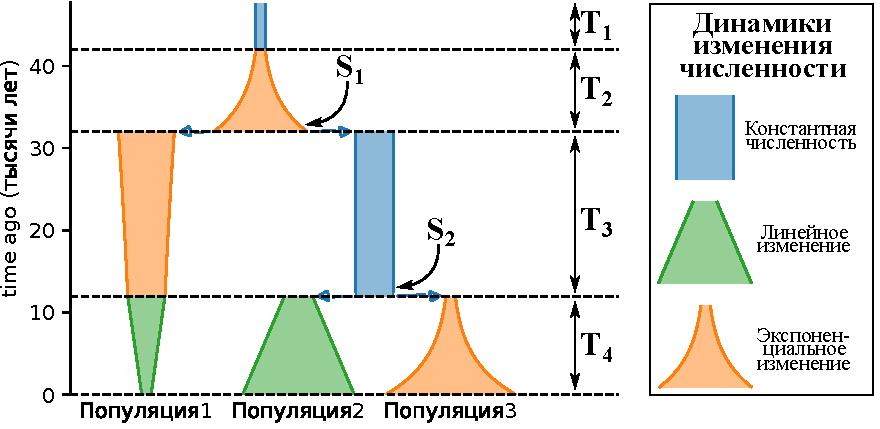
\includegraphics[width=\linewidth]{part2/auto_model/dem_model_col.pdf}
  \captionof{figure}{Пример демографической модели со структурой (2,1,1)
}
  \label{fig:exaple_of_model_plot}
\end{figure*}

Теперь мы можем определить понятие \textbf{структуры демографической модели}.
В случае двух популяций, структура модели будет включать число временных интервалов, которые происходят до и после единственного события разделения. В случае трех популяций структура включает число временных интервалов до первого разделения, число интервалов между первым и вторым разделениями и число интервалов после второго разделения.
Например, предположим, что мы наблюдаем три популяции.
В начале существовала предковая популяция ($P_A$), и эта популяция начала расти в эффективном размере.
Затем произошло разделение этой предковой популяции на две дочерние популяции ($P_1$ и $P_2$), которые изменились в  размере в течение одного интервала времени, за которым последовало разделение второй популяции (на $P_{2a}$ и $P_{2b}$), в результате чего появились три популяции-потомка, изменившиеся в течение одного последующего интервала времени. 
Структура такой модели описвается как (2,1,1) (Рисунок~\ref{fig:exaple_of_model_plot}).
Простейшие структуры модели были бы для двух популяций --- (1,1), и для трех популяций --- (1,1,1).

Рисунок~\ref{fig:exaple_of_model_plot} демонстрирует модель демографической истории трех популяций со структурой.
На рисунке отмечены четыре временных интервала: $T_1$, $T_2$, $T_3$ и $T_4$, и два расщепления популяций: $S_1$ и $S_2$.
Структура этой модели имеет вид (2,1,1), поскольку $T_1$ и $T_2$ --- это временные интервалы для предковой популяции, за которой последовало разделение $S_1$, $T_3$ --- это временной интервал для двух популяций, а $T_4$ --- это временной интервал для трех популяций после второго раскола $S_2$.
Разные динамики изменения численности в модели изображены следующими цветами: константная численность соответствует синему цвету, линейное изменение --- зеленому, и экспоненциальное изменение --- оранжевому цвету.
Первый временной интервал $T_1$ имеет один параметр --- размер предковой популяции.
Временной интервал $T_2$ имеет следующие параметры: время этого интервала, размер предковой популяции в конце и динамика изменения размера.
Временные интервалы $T_3$ и $T_4$ для каждой популяции будут содержать те же параметры плюс миграции между популяциями. 
События разделения $S_1$ и $S_2$ характеризуются долей размера разделения.

Более формально, структура модели --- это последовательность вида $S^* = \{s^*_i\}_{i=1}^P, \quad s^*_i \in \mathbb{N}$, где $P \in \{2, 3\}$ --- число популяций.
В этом случае число параметров $N_\Theta(S^*)$ демографической модели со структурой $S^*$ будет определяться следующим образом:

\begin{equation}N_\Theta (S^*) = (P-1)  + \sum_{i = 0}^P{N_\Theta^i(s^*_i)},\quad
\text{where} \quad N_\Theta^i(s^*_i) = \begin{cases}
        3(s^*_1 - 1), & \text{if } i = 1,\\
        7s^*_2, & \text{if } i = 2,\\
        13s^*_3, & \text{if } i = 3.
        \end{cases} 
\end{equation}

Слагаемое $(P - 1)$ соответствует числу параметров разбиения, а $\sum_{i = 0}^P{N_\theta^i(s^*_i)}$ --- числу параметров временных интервалов.
Такое число параметров $N_\Theta (S^*)$ справедливо для разработанного генетического алгоритма, но число конечных параметров модели другое.
Во время локального поиска, который происходит после генетического алгоритма, динамика изменения численности популяции фиксируется и конечное число параметров $\overline{N}_\Theta (S^*)$ составляет:

\begin{equation}\overline{N}_\Theta (S^*) = (P-1)  + \sum_{i = 0}^P{\overline{N}_\theta^i(s^*_i)},\quad 
\text{where} \quad \overline{N}_\Theta^i(s^*_i) = \begin{cases}
        2(s^*_1 - 1), & \text{if } i = 1,\\
        5s^*_2, & \text{if } i = 2,\\
        10s^*_3, & \text{if } i = 3.
        \end{cases}
\end{equation}

Таким образом, мы можем однозначно интерпретировать демографическую модель по списку параметров и ее структуре, зафиксировав для каждого временного интервала определенный порядок параметров.\\

\section{Алгоритм увеличения структуры и автоматического перебора расширенных моделей демографической истории}

Нам необходимо иметь возможность увеличивать сложность структуры демографической модели, чтобы найти оптимальное решение.
Для того, чтобы увеличить структуру модели выбирается временной интервал в этой структуре, который делится на два интервала равной длины.
Временной интервал выбирается произвольно, исходя из того, что новая структура $S^*$ не должна стать больше конечной $S^F$ по одному из значений: $s^*_k \leq s^F_k,\quad \forall k \in [1,P]$.
Значения параметров вновь образованных временных интервалов рассчитываются по родительскому: размер популяции в конце первого временного интервала равен размеру в середине родительского временного интервала, а численности популяций в конце второго временного интервала равны численностям родительского.
При этом время обоих интервалов равно половине родительского времени, а миграция между популяциями и демографическая динамика изменения размера популяции остаются неизменными.
По сути, демографическая модель имеет больше параметров после увеличения ее структуры, однако история и вероятность остаются прежними.

Таким образом был предложен новый метод для автоматического перебора моделей демографической истории популяций.
Он требует эффективный алгоритм глобальной оптимизации, который способен находить как непрерывные так и дискретные параметры, а также алгоритм локальной оптимизации.
Алгоритм локального поиска используется после запуска глобальной оптимизации для дополнительного более аккуратного уточнения значений непрерывных параметров нашей модели.
Поэтому для их использования динамики изменения численности в расширенной модели со структурой фиксируются, так как они являются дискретными параметрами.
Один из алгоритмов глобальной оптимизации, подходящий для метода автоматического поиска демографической истории, а именно генетический алгоритм, был разработан в данной работе и описан в разделе~\ref{sec:part2:genenic_algorithm}.
В качестве алгоритмов локального поиска мы предлагаем такие методы как:
\begin{itemize}
    \item BFGS,
    \item L-BFGS-B,
    \item Метод Пауэлла,
    \item Метод Нилдера-Мида.
\end{itemize}
Эти методы используются в существующих библиотеках \dadi, \moments, \momentsLD для вывода параметров модели демографической истории популяций и показали свою эффективность при поиске локального оптимума.

\begin{figure}
    \centering
    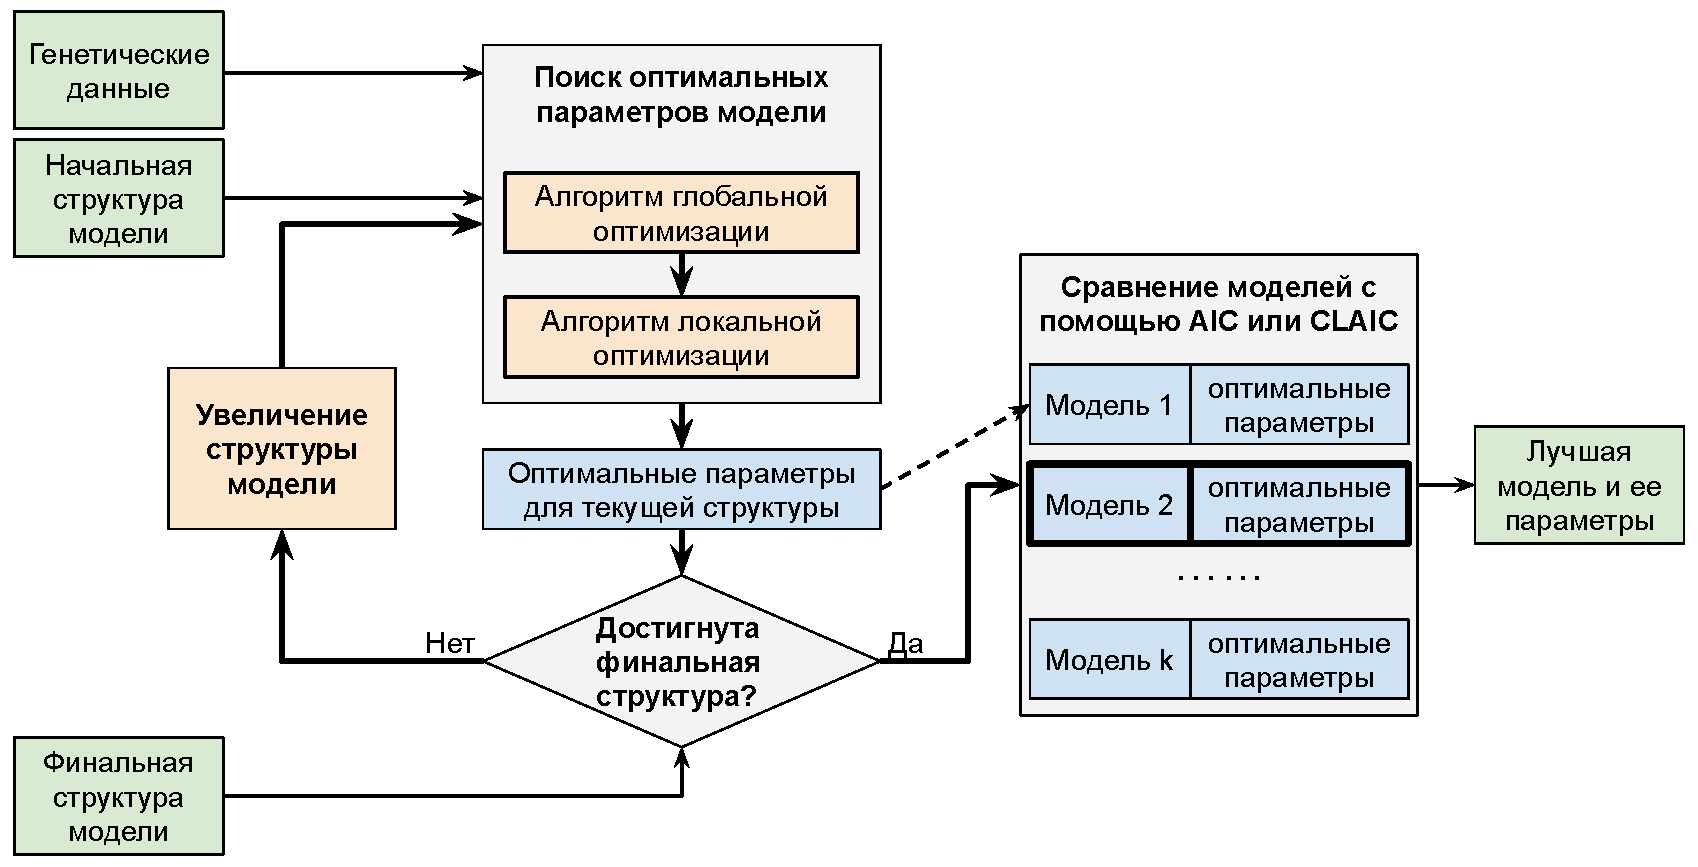
\includegraphics[width=\textwidth]{images/part2/auto_model/general_scheme_rus.pdf}
    \caption{Схема метода автоматического поиска модели демографической истории и ее параметров}
    \label{fig:part2:auto_model:algorithm}
\end{figure}

Таким образом алгоритм принимает на вход две структуры модели демографической истории: начальную и финальную.
С помощью алгоритма глобальной оптимизации происходит поиск параметров модели с начальной структурой.
Затем непрерывные параметры дополнительно уточняются с использованием локальной оптимизации.
Полученные значения параметров сохраняются как оптимальные для модели с данной структурой для сравнения моделей в конце.
После этого происходит увеличение структуры и поиск параметров новой модели с использованием той же комбинации алгоритмов глобальной и локальной оптимизации.
Посдений шаг повторяется до тех пор, пока не будет достигнута финальная структура.
В качестве ответа алгоритм предлагает финальные истории для моделей с разными структурами, которые дополнительно сравниваются с помощью AIC или CLAIC для выбора наилучшего решения.

Схема разработанного метода автоматического поиска модели демографической истории популяций и ее параметров представлен на рисунке~\ref{fig:part2:auto_model:algorithm}.
Зеленым цветом выделены входные и выходные данные.
На вход метод принимает генетические данные, а также начальную и конечную структуры расширенной модели.
На выход мы получаем модель демографической истории с оптимальными параметрами, которая наилучшим образом описывает генетические данные.
Псевдокод разработанного алгоритма представлен в Листинге~\ref{alg:part2:auto_search}.